% Put all your plots in the plots folder. If required, make further folders.

\documentclass[a4paper]{article}
\usepackage[colorlinks=True, linkcolor=blue, urlcolor=blue]{hyperref}
\usepackage[]{geometry}
\usepackage{amsmath}
\usepackage{amssymb}
\usepackage{graphicx}
\usepackage{listings}
\usepackage{color}
\usepackage{algorithmic}
\usepackage{float}
\usepackage[table,xcdraw]{xcolor}
\usepackage{longtable}

\definecolor{string}{RGB}{170, 55, 241}
\definecolor{comments}{RGB}{6, 186, 72}
\lstset{language=Matlab, numbers=left,
	breaklines=true, commentstyle=\color{comments},
	stringstyle=\color{string}, keywordstyle=\color{blue},
	emph=[1]{ylim,xlim, movmean, islocalmin, isoutlier, vertcat}, emphstyle=[1]\color{blue}}


\title{Processor Architecture assignment 2\\\Large{Exploring caching algorithms using the ChampSim simulator}}
\author{1. Sai Manish Sasanapuri (IMT2018520)\\ 2. Shubhayu Das (IMT2018523)\\  3. Veerendra S. Devaraddi (IMT2018529)}

\begin{document}
\maketitle
\tableofcontents
\pagebreak

% General Introduction
\section{Introduction}
    In this assignment, we explore a variety of algorithms that can be used in the cache hierarchy in modern processors. We have implemented the following:
    \begin{enumerate}
        \item Manish - Best Offset Prefetching - a data prefetching algorithm
        \item Shubhayu - Bimodal and Dynamic insertion policies - 2 LLC cache insertion and replacement policies
        \item Veerendra - 3 different variations of gshare, pshare and a tournament predictor, based on gshare and pshare
    \end{enumerate}
    
    For all our experiments, we used the \href{https://github.com/ChampSim/ChampSim}{ChampSim cache simulator}. We used the default cache configurations, on a single core processor. All simulations were run with 100M instructions for warmup, followed by 100M instructions of actual execution.\\
    
    We utilized the following trace files, which were obtained from \href{http://hpca23.cse.tamu.edu/champsim-traces/speccpu/}{here}:
    \begin{itemize}
        \item 400.perlbench-41B.champsimtrace.xz (178MB)
        \item 410.bwaves-945B.champsimtrace.xz (66MB)
        \item 603.bwaves\_s-1080B.champsimtrace.xz (50MB)
        \item 638.imagick\_s-824B.champsimtrace.xz (190MB)
        \item 403.gcc-48B.champsimtrace.xz (38MB)
        \item 458.sjeng-1088B.champsimtrace.xz (218MB)
        \item 625.x264\_s-20B.champsimtrace.xz (57MB)
        \item 657.xz\_s-56B.champsimtrace.xz (90MB)
    \end{itemize}
    
    For redundancy, here is our cache configuration:
    \begin{center}
        \begin{table}[h]
            \begin{tabular}{|c|c|c|c|}
            \hline
            \textbf{Cache}          & \textbf{\#ways}   & \textbf{\#sets} & \textbf{latency(in cycles)} \\ \hline
            L1 instruction & 8        & 64     & 4                  \\ \hline
            L1 Data        & 64       & 12     & 5                  \\ \hline
            L2             & 1024     & 8      & 10                 \\ \hline
            LLC            & 2048/CPU & 8      & 20                 \\ \hline
            \end{tabular}
        \end{table}
    \end{center}
    
    Our code and all result files can be found in \href{https://github.com/vsdevaraddi/PA_Champsim_assignment}{this GitHub repository}.

\pagebreak
% Manish
\section{Cache prefetching algorithm}
 \subsection{Introduction}
    Prefetching is a method to predict the data needed in future and fetch them into cache before it is requested by the program. Prefetching reduces compulsory misses and reduces memory access latency when the prefetch accuracy is high and prefetch is done at correct time. We have two types of prefetching : Hardware prefetching and Software prefetching. In software prefetching compiler analyzes the code and insert prefetch instruction during compilation. In hardware prefetching dedicated hardware observes past load/store access and prefetches the data. In this assignment we were mainly insterested in hardware prefetchers. Prefetching can be done at any cache level. Level-1 (L1)
    and level-2 (L2) prefetching lead to different possibilities and
    tradeoffs, hence different sorts of prefetchers. L1 caches have stronger capacity and bandwidth constraints than L2/L3 caches. L1 caches do not tolerate inaccurate prefetches, while L2/L3 caches do to a certain extent. Best-Offset prefetching is intended for L2 prefetching which is implemented in Champsim.
    
    \subsection{Common existing Prefetchers}
        \subsubsection*{Next-Line prefetcheing method}
            Next-line prefetching one of the simplest prefetching method. In this method we prefetch line X+1 when line X is accessed. 
            \\ Next-line prefetching is easy to implement, but does now work well with all access patterns.
        
        \subsubsection*{Stride prefetchering method}
            Stride prefetchers tries to identify, among load and store instructions, those that access memory with a constant stride [1, 7, 31]. Stride prefetchers usually have a table indexed with load/store PCs. An important feature of stride prefetchers is that they issue a prefetch request only if there is a certain confidence that the prefetch will be useful. However, stride prefetchers are more easily implemented at the L1, as they need to see all the memory instructions, including those that hit in the DL1, and preferably in program order.
            
        \subsubsection*{Stream prefetching method}
            Stream prefetching exploits sequential streams, like next-line prefetching, but tries to improve prefetch timeliness and decrease useless prefetches by prefetching several successive lines into a stream buffer when a stream has been detected. Only when a demand access hits on the stream buffer head is the prefetched line moved into the cache (hence reducing cache pollution), and a new line is prefetched to keep the stream buffer full. Several stream buffers are needed for good performance on interleaved streams.
            
        \subsubsection*{Offset Prefetching method}
        Offset prefetching is a generalization of next-line prefetching. When a line of address X is requested by the core, an offset prefetcher prefetches line X+D, where D is the prefetch offset. The optimal offset value is not the same for all applications. 
        
        \subsubsection*{IP- Stride prefetcher}
        The stride prediction from the IP(instruction pointer) table when the
        IP-delta-based sequence predictor cannot offer a prediction due to
        IP-delta table misses or low-confidence predictions. This strategy
        avoids loss in coverage. This prediction comes for free without any
        additional overhead, since the IP table has to be looked up anyway.
        After the FIFO list of the matching IP table entry is updated by
        inserting the current delta, if the last (youngest) two deltas in the
        FIFO list are identical, this delta is used for generating a prefetch
        sequence of length d in the cases when the IP-delta table cannot
        offer a prediction due to miss or low confidence. We also employ
        this delta predicted from the IP table to complete an otherwise
        prematurely terminated prefetch sequence due to a low confidence
        delta in the IP-delta table’s predicted sequence.
        
    \subsection{My Implementation}
        Idea is to implement full-fledged offset prefetcher has an offset selection mechanism for setting dynamically the offset depending on application behavior.
        Best offset prefetching method : referred from \href{https://hal.inria.fr/hal-01254863}{Pierre Michaud. Best-Offset Hardware Prefetching. International Symposium on High-Performance Computer Architecture, Mar 2016, Barcelona, Spain.}
        \\ 
        
        \subsubsection*{Best offset prefetching}
            Overview of working of Best offset prefetching, when a read request for line X accesses the L2 cache, if this is a miss or a prefetched hit and if X and X + D lie in the same memory page, a prefetch request for line X+D is sent to the L3 cache.
            
        \begin{figure}[h]
        \centering % centering figure
        %\scalebox{0.8} % rescale the figure by a factor of 0.8
        {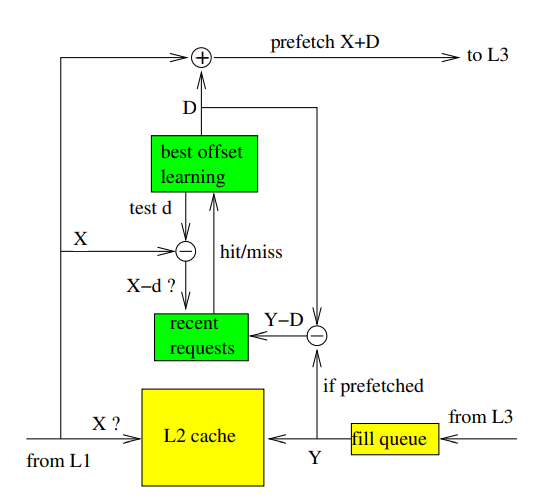
\includegraphics[width = 0.8 \linewidth]{images/Manish/block_diagram.png}} % importing figure
        \caption{Schematic view of a BO prefetcher}
        \label{fig:exm} % labeling to refer it inside the text
        \end{figure}
        
        \subsubsection*{Best-offset learning}
        The prefetch offset D is set automatically and dynamically, trying to adapt to the application behavior, which may vary over time. The best-offset learning algorithm tries to find the best prefetch offset by testing several different offsets. An offset d is potentially a good prefetch offset if, when line X is accessed, there was in the recent past a previous access for line X - d. However, the fact that X - d was recently accessed is not sufficient for guaranteeing that line X would have been prefetched in time. We want prefetches to be timely whenever possible. I.e., for d to be a good prefetch offset for line X, line X - d must have been accessed recently, but not too recently.\\
        
        Ideally, the time between the accesses to lines X - d and X should be greater than the latency for completing a prefetch request. If line X - d is in the RR table, it means that a prefetch request for line X - d + D was recently issued and has been completed. Therefore, if a prefetch request had been issued with offset d instead of D, it would have been a prefetch for the line X currently accessed, and this prefetch would have been timely (assuming that the latency of fetching line X equals the latency of fetching line X - d + D).\\
        
        Besides the RR table, the BO prefetcher features an offset list and a score table. The score table associates a score with every offset in the offset list. The score value is between 0 and SCOREMAX = 31. The prefetch offset is updated at the end of every learning phase. A learning phase consists of several rounds. At the start of a learning phase, all the scores are reset to 0. On every eligible L2 read access (miss or prefetched hit), we test an offset $d_i$  from the list. If X - $d_i$ hits in the RR table, the score of offset $d_i$ is incremented. During a round, each offset in the list is tested once.\\

        When all the offsets in the list have been tested, the current round is finished, and a new round begins from first offset in offset list again. The current learning phase finishes at the end of a round when either of the two following events happens first: one of the scores equals SCOREMAX, or the number of rounds equals ROUNDMAX (a fixed parameter). When the learning phase is finished, we search the best offset, i.e., the one with the highest score. This offset becomes the new prefetch offset, and a new learning phase start.

        
     \subsection{Results}
        \begin{enumerate}
            \item My Best of set prefetcher implementation is failing in updating the new best offset when changing from current learning phase to new learning phase.
        \end{enumerate}
        
        The below plot is the analysis of performance of prefetching methods where the used branch predictor is bimodal and used replacement policy is DRRIP.
        
        \begin{figure}[H]
        \centering % centering figure
        %\scalebox{0.8} % rescale the figure by a factor of 0.8
        {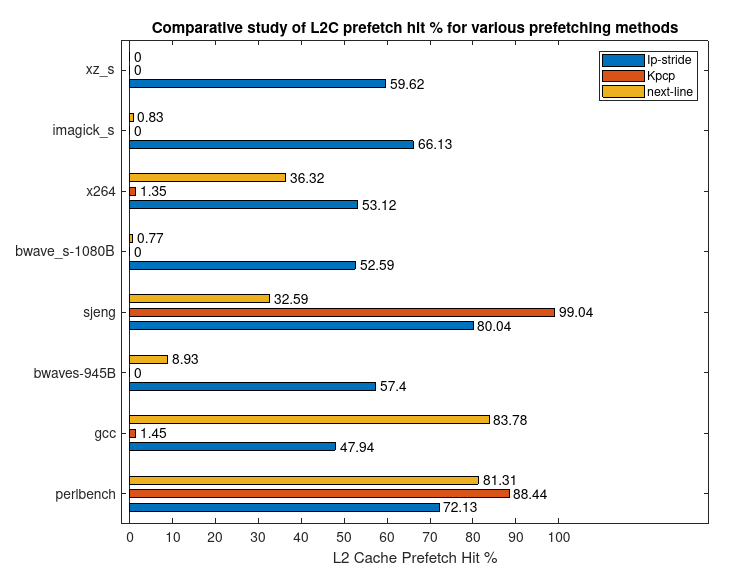
\includegraphics[width = 0.8 \linewidth]{images/Manish/plot.png}} % importing figure
        \caption{Prefetcher accuracy for various prefetching methods}
        \label{fig:exm} % labeling to refer it inside the text
        \end{figure}
        
     \subsection{Conclusion}
      \begin{enumerate}
            \item Here from the plot it is difficult to say that among the 3 prefetching methods one is best prefetching method.
            \item For traces 1 and 4 Kpcp prefetcher has highest prefetch hit \% 
            \item In general Ip-Stride prefetcher has shown reasonable performance for any trace file.
            \item Where as Kpcp  and next-line prefetchers were sometimes either performing exteremly will for some trace file and sometimes very bad for some trace files.
            \item Trace files 3,5,7,8 might have irregular data access that is why prefetch hit rate is too less for next-line prefetching method.
        \end{enumerate}
     
\pagebreak
% Shubhayu
\section{Cache replacement policies}
    \subsection{Introduction}
        The data in the cache must be updated to be the most relevant to the process in execution. Old blocks of data can form dead regions in the cache, reducing its effective size. To handle this problem, cache replacement algorithms/policies are used. To detect which blocks are to be replaced by incoming data, the algorithm maintains some record of the memory access pattern. These algorithms are typically implemented in the last level cache(LLC), which is large enough to effectively use these algorithms without any significant overheads.\\
    
        The simplest policy is to replace the \textit{least recently used(LRU)} cache block. As simplistic as it sounds, it still works pretty well for a number of daily execution processes.
        
    \subsection{Need for other predictors}
        LRU fails to be effective when the working set is larger than the cache size. The useful data is constantly replaces and re-fetched, leading to a phenomenon called \textit{cache thrashing}(essentially, all misses). Further, many of the cache lines are never actually accessed before being replaced.\\
        
        To overcome this problem, any new algorithm must:
        \begin{enumerate}
            \item Carry forward some of LRU's effectiveness
            \item Have a unique \textit{cache insertion} method
            \item Have an effective \textit{victim selection} policy
        \end{enumerate}
        
    \subsection{My implementation}
        I referred to \href{https://people.csail.mit.edu/emer/papers/2007.06.isca.dip.pdf}{Adaptive Insertion Policies for High Performance Caching, Qureshi et. al., ISCA 2007} for their work of 3 different branch predictors. These can be summarized as follows:
        \begin{table}[h]
            \begin{tabular}{|c|c|c|c|}
            \hline
            \textbf{Method} & \textbf{Insertion policy}                                                                                  & \textbf{Victim selection policy}   & \textbf{Update policy}                                                                                                                                \\ \hline
            LRU    & In MRU position                                                                                   & Entry with lowest recency & \begin{tabular}[c]{@{}c@{}}Recency of entry\\  always decreases\end{tabular}                                                                 \\ \hline
            LIP    & In LRU position                                                                                   & Entry with lowest recency & \begin{tabular}[c]{@{}c@{}}Promoted from LRU\\  to MRU only on reuse\end{tabular}                                                            \\ \hline
            BIP    & \begin{tabular}[c]{@{}c@{}}In LRU, but some entered\\  into MRU with low probability\end{tabular} & Entry with lowest recency & \begin{tabular}[c]{@{}c@{}}Promoted from LRU\\  to MRU only on reuse. Entries\\ which are not at LRU decrement\\  their recency in every cycle\end{tabular} \\ \hline
            DIP    & \begin{tabular}[c]{@{}c@{}}Dynamically choosing\\ between BIP and LIP\end{tabular}                & Entry with lowest recency & \begin{tabular}[c]{@{}c@{}}Depending on policy\\  of a cache block\end{tabular}                                                              \\ \hline
            \end{tabular}
        \end{table}
        
        {\centering(\textit{LIP - LRU Insertion Policy, BIP - Bimodal Insertion Policy, DIP - Dynamic Insertion Policy, MRU - Most Recently Used})}\\
        
        The DIP method defined above is actually called DIP-Global, which implements both BIP and LIP. However, this is not practical because it is extremely resource intensive. As an alternative, the authors came up with DIP-Set Dueling(DIP-SD). In DIP-SD, the cache sets are divided into three categories:
        \begin{enumerate}
            \item Sets dedicated to LIP
            \item Sets dedicated to BIP
            \item follower sets
        \end{enumerate}
        
        There is a global counter called PSEL, which keeps track of the most successful policy. Depending on the MSB of the PSEL, any access to the follower cache sets follow BIP or LIP. In the paper(and my implementation), PSEL is a 10 bit saturating counter, shared across all the ways. In my implementation, for every 64 sets, one set is dedicated to LIP and another is dedicated to BIP. For a more detailed explanations and the original results, please refer to the paper above(section 4, 5 and figure 10, 11). I am leaving out details like the bimodal throttle parameter used in BIP, because they are already well described in the paper.
        
        \subsection{Results}
            I ran my simulations based on the details mentioned in Section 1. The CPU model used a bimodal branch predictor, with no prefetching is any level of the cache. I have calculated the overall LLC cache miss percentage, for 5 different cache replacement policies. It is a little amusing to see LRU perform the best in most of the benchmark traces. In general, SRRIP and DRRIP hold their own pretty well. BIP seems to outperform DIP, which is rather unexpected.
            
            \begin{center}
                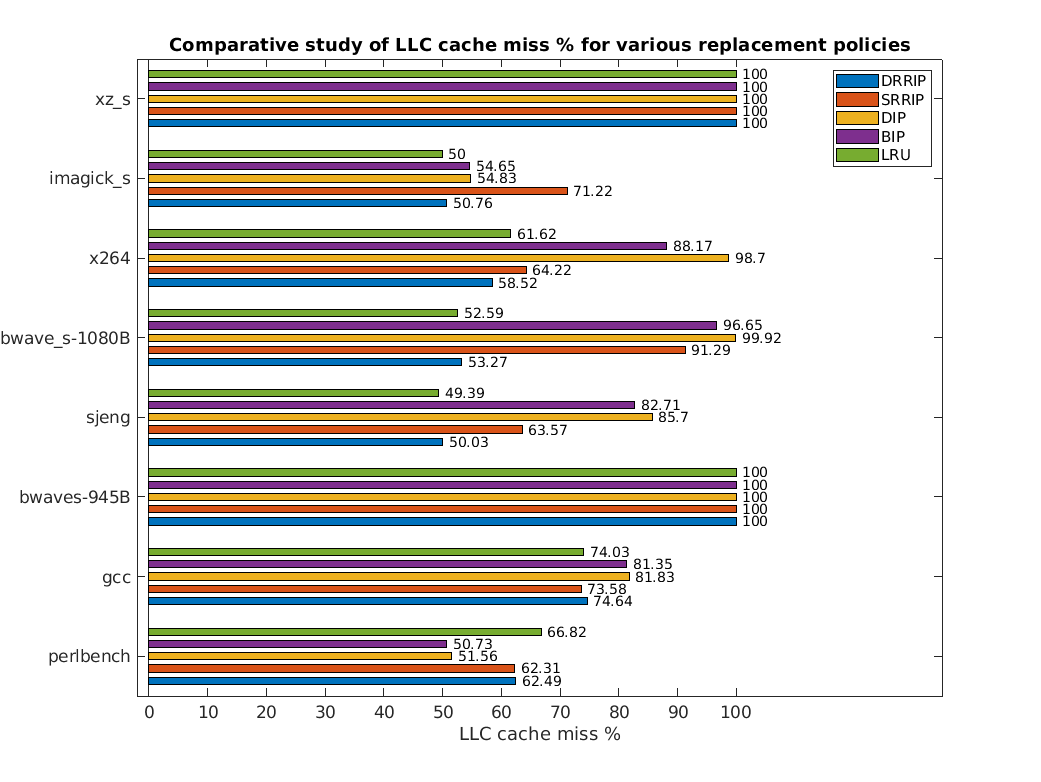
\includegraphics[width=\linewidth]{images/shubhayu/LLC.png}
                \title{Results from my simulations in ChampSim. The CPU has a single core, with no prefetching and a bimodal branch predictor.(\textit{lower value along x-axis is better.})}
            \end{center}
            
            Another important observation: the performance of the policies in these benchmarks is a rather poor measure of their performance. In two of the benchmarks, all LLC accesses lead to misses. To get a more conclusive result, we need to test over a larger variety of benchmarks, for more number of instructions(I only ran for 100M instructions, because it is very time consuming).\\
            
            To verify the validity of the results above, I ran the simulations again. This time, I am using the Gshare branch predictor, with next-line prefetching for L1D, L1I and LLC, and SPP\_DEV prefetching for L2C. The results show a similar trend. The difference in the values is due the difference in the cache accesses due to the prefetches.
            
            \begin{center}
                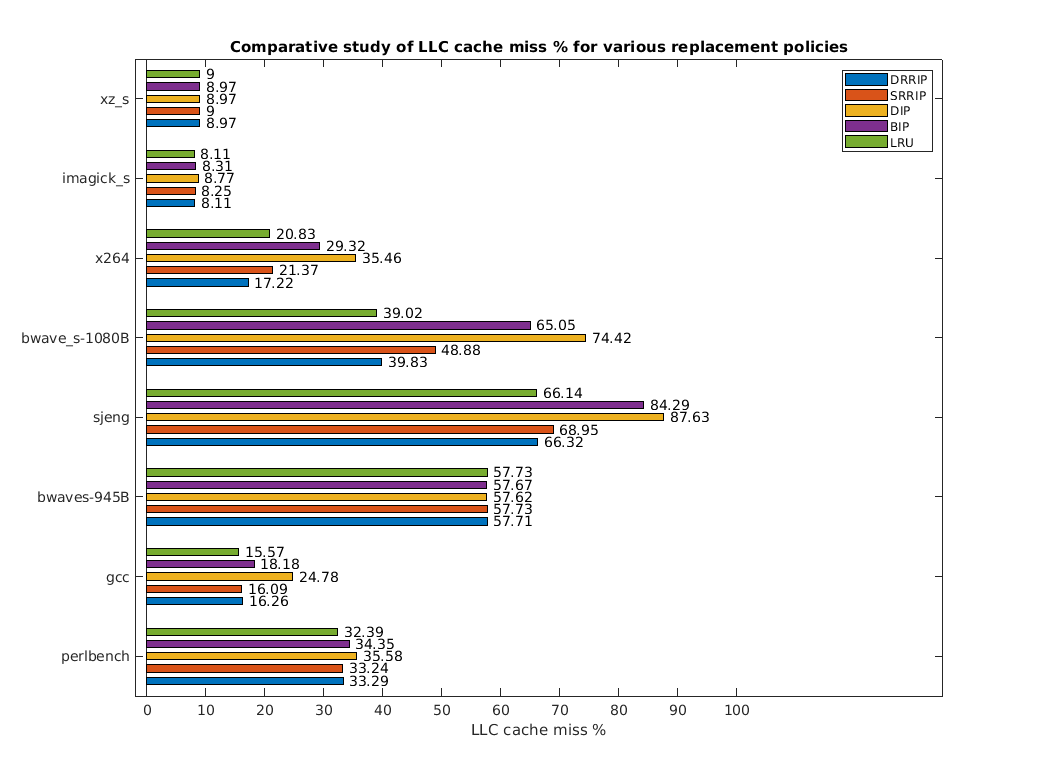
\includegraphics[width=\linewidth]{images/shubhayu/LLC_gshare.png}
                \title{Results from my simulations using gshare, different prefetching schemes for all the caches, and a single core.(\textit{lower value along x-axis is better.})}
            \end{center}
            
            With a prefetcher in place, just analyzing the overall LLC misses is not fair. What I should ideally analyze is the number of misses, in the valid prefetches(prefetches that brought in data that was used in the future). However, there is no metric to measure this in ChampSim.

        \subsection{Conclusion and other explorations}
            From the benchmarks, I ran, it is evident that neither BIP nor DIP-SD can reliably out-perform the LRU policy. My reasoning is that in BIP, there is not effective aging mechanism. A large majority of the entries are always stuck at the LRU position. As a result, we don't know if their presence in the cache is useful or not. Similarly. DIP-SD suffers from the same problem: LIP has \textit{no} aging mechanism whatsoever, and BIP algorithm's problem is mentioned earlier. As a result, DIP-SD algorithm isn't significantly better in my tests. In my opinion, a better implementation would have to enter new elements with a recency of $\displaystyle\frac{MAX\_LRU\_VALUE}{2}$. The aging mechanism could combine those of LRU and BIP - decrement recency by one in every cycle, except when accessed. On access, the recency counter can be incremented by one.\\
            
            I additionally explored and tried out RRIP(Re-Reference Interval Prediction) based replacement policies(Static-RRIP and Dynamic-RRIP, SRRIP and DRRIP respectively). These policies perform uniformly better than LRU, BIP and DIP, with a few exceptions. The calculation of the re-reference interval seems to address the aging problem that BIP/DIP have. I referred to: \href{https://people.csail.mit.edu/emer/papers/2010.06.isca.rrip.pdf}{High Performance Cache Replacement Using Re-Reference Interval Prediction (RRIP), Jaleel et. al., ISCA 2010} for RRIP based LLC cache replacement policies. (Un)fortunately, these were already implemented in ChampSim, so I didn't implement them on my own.
        
\pagebreak
% Veerendra
\section{Branch predictor}
    \subsection{Introduction}
        One way of improving the performance or the IPC(Instructions Per Cycle) of a processor, is by predicting the branch outcomes. Predicting the branch outcome would help to fetch and continue with an new appropriate instruction, therefore utilising the cycles till  the actual outcome of the branch instruction is computed. As the result of which, the IPC of the processor increases over a processor with no branch prediction.
    \subsection{Examples of Branch predictors}
        \subsubsection{Gshare}
            Gshare branch predictor uses a global history register which stores the true outcomes of its previous branch instructions. It has branch history table which stores the states of a 2-bit FSM. Gshare uses global history register and PC of the instruction to index into branch history table. Generally Gshare uses a unbiased FSM which we can refer as A2, as shown in the diagram below
            \begin{figure}[ht]
                \centerline{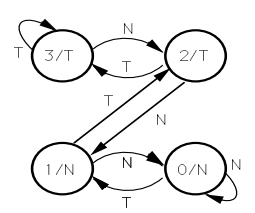
\includegraphics[width= 4cm]{images/veerendra/gshare_a2.png}}
                \caption{Gshare unbiased FSM, A2}
                \label{fig_gshare_a2}
            \end{figure}
        \subsubsection{Gshare A1}
            Gshare A1 is a variant of Gshare(A2) with an FSM which records the previous two branch results of a specific branch instruction with a specific global history. This previous history can be used to predict the branch. The FSM of A1 is \\
            \begin{figure}[ht]
                \centerline{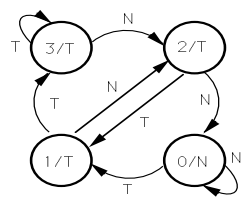
\includegraphics[width= 4cm]{images/veerendra/gshare_a1.png}}
                \caption{Gshare bieased FSM, A1}
                \label{fig_gshare_a1}
            \end{figure}
            \\
            If the state of the FSM is 3 then the previous two results of the branch(with specific global history) is taken and taken. If the state of the FSM is 2 then the previous two results of the branch is not-taken and taken. If the state of the FSM is 1 then the previous two results of the branch is taken and not-taken. If the state of the FSM is 0 then the previous two results of the branch is not-taken and not-taken.\\
            If either one or both of the previous two results of the branch is/are taken then the prediction is taken. If both the previous two results are not-taken then the prediction is non-taken. Therefore there is a bias towards taken.    
        \subsubsection{Gshare A3}
            Gshare A3 is another variant of Gshare(A2) with FSM which is similar to A2 but directly jumps to state 3 upon taken from state 1 and directly jumps to state 0 upon not-taken from state 2. Therefore A3 unlike A2, directly goes to highest confident states(0,3) when there is a mis-prediction from low confident states(1,2). This FSM is symmetric, as the result predictions are unbiased.
            The FSM of A3 is
            \begin{figure}[ht]
                \centerline{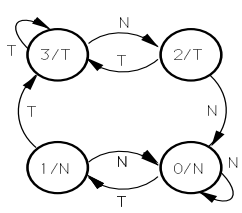
\includegraphics[width= 4cm]{images/veerendra/gshare_a3.png}}
                \caption{Gshare unbiased FSM, A3}
                \label{fig_gshare_a3}
            \end{figure}
        \subsubsection{Gshare A4}
            Gshare A4 is another variant of Gshare(A2) with FSM which is similar to A3 but its biased towards taken because unlike A3 it directly jumps to state 3 upon taken from state 1 only. Therefore A4 like A3, directly jumps to highest confident taken state(3) when there is a mis-prediction from low confident not-taken state(1), but A4 unlike A3 will  \textbf{not} directly jump to highest confident not-taken state 0 when there is a mis-prediction from low confident taken state(2). This FSM is biased towards taken because of asymmetry. Ths FSM of A4 is
            \begin{figure}[ht]
                \centerline{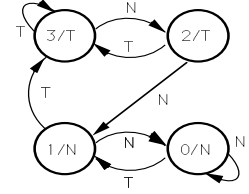
\includegraphics[width= 4cm]{images/veerendra/gshare_a4.png}}
                \caption{Gshare biased FSM, A4}
                \label{fig_gshare_a4}
            \end{figure}
            
        \subsubsection{Pshare}
            Pshare is branch predictor with a private history space for each instruction in a set, in a Per-branch History Table. PHT can be indexed by the PC of the instruction. Pshare has a branch history table which stores the states of a 2-bit FSM. Pshare uses both PHT entry and PC of the instruction to index into branch history table.
            Generally pshare uses a unbiased FSM, as shown in the below diagram
            \begin{figure}[ht]
                \centerline{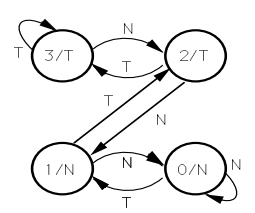
\includegraphics[width= 4cm]{images/veerendra/gshare_a2.png}}
                \caption{ Pshare FSM}
                \label{fig_pshare_fsm}
            \end{figure}
            
        \subsubsection{Tournament predictor}
            Pshare performs better then Gshare when coherency exists in the results of a branch over the time. Gshare perform better than Pshare when coherency exists with the results of previous branches. In order to explore both the coherencies, pshare and gshare can be combined.\\  
            \\Tournament predictor uses either Pshare or Gshare to predict a branch. It has a meta table which stores the state of a FSM for many instructions, which is used to select either Gshare or Pshare.\\
    \subsection{Comparison between predictors}
        \subsubsection{Gshare and its variants}
            Gshare  A4 would perform better than A3 when the trace is biased towards  taken because A4 is a modification of A3 which is biased towards taken.\\
            \\Gshare A1 performs better than rest of the Gshare variants when the trace contains branches which follows one of the following patterns: NNN, NTT, TNT or TTT over time.
        \subsubsection{Gshare and Pshare}
            Pshare performs better then Gshare when coherency exists in the results of a branch over the time. Gshare perform better than Pshare when coherency exists with the results of previous branches.
        \subsubsection{Tournament, Gshare and Pshare}
            Tournament always perform better than Gshare as well as Pshare.\\
    \subsection{Results}
        \begin{figure}[ht]
            \centerline{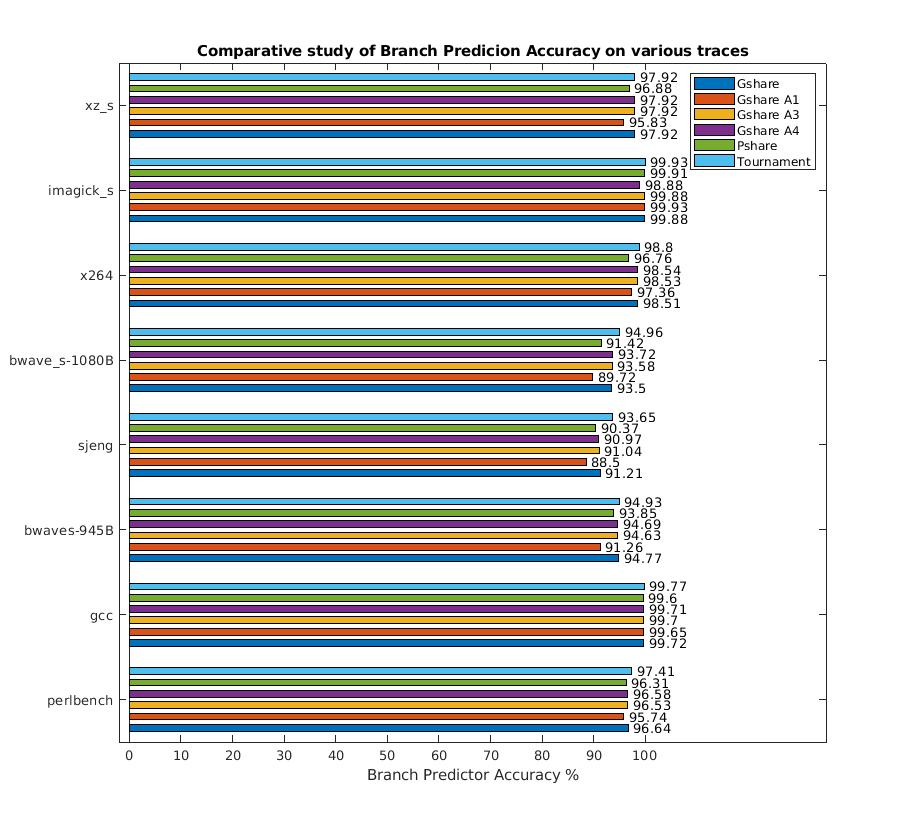
\includegraphics[width= \linewidth]{images/veerendra/final_accuracy}}
            \caption{Branch Predictor accuracy of branch predictors on various traces}
            \label{fig_branch_predictor_accuracy}
        \end{figure}
    
    \subsection{Conclusions}
        \begin{enumerate}
            \item  Tournament predictor always performs better than rest of the predictors considered here.
            \item Gshare performs better than Pshare for majority of traces
            \item Most of the traces do not show 'taken' bias to a extent such that Gshare A4 out performs others. If a trace is not a 'taken' biased then performance of Gshare A4 actually reduces. We can conclude that unbiased FSMs have better performance in an unknown environment.
            \item Gshare A1 rarely performs better than other variants because it keeps track of patterns which includes only two previous results while other variants use "confidence" metric to predict.
            
        \end{enumerate}

\pagebreak
\section{References}
    \begin{enumerate}
        \item  Yeh and Patt, “Alternative Implementations of Two Level Adaptive Branch Prediction”
        \item \href{https://people.csail.mit.edu/emer/papers/2007.06.isca.dip.pdf}{Adaptive Insertion Policies for High Performance Caching, Qureshi et. al., ISCA 2007}
        \item \href{https://people.csail.mit.edu/emer/papers/2010.06.isca.rrip.pdf}{High Performance Cache Replacement Using Re-Reference Interval Prediction (RRIP), Jaleel et. al., ISCA 2010}
        \item Pierre Michaud. Best-Offset Hardware Prefetching. International Symposium on High-Performance Computer Architecture, Mar 2016, Barcelona, Spain.
    \end{enumerate}
        
            
\end{document}
